\documentclass[xetex,notheorems,hyperref={pdfpagelabels=true},xcolor={table},aspectratio=169]{beamer}
\usetheme{dnv}

\usepackage{booktabs}
\usepackage[scale=2]{ccicons}

\usepackage[style=american]{csquotes}

\usetikzlibrary{decorations.pathreplacing, decorations.pathmorphing,calc,arrows,positioning}



%%% enable notes on second screen
%\usepackage{pgfpages}
%\setbeameroption{show notes on second screen=right}
%\setbeamertemplate{note page}[compress]

	
%%%%%%%%%%%%%%%%%%%%%%%%%%%%%%%%%%%%%%%%%%%%%%%%%%%
%%%%	define content of title page
%%%%%%%%%%%%%%%%%%%%%%%%%%%%%%%%%%%%%%%%%%%%%%%%%%%
\def\talkTitle{Seminar on Cybersecurity of Rail transport}
\def\talkShortTitle{TS 50701 }
\def\talkSubtitle{TS 50701 \& IEC/ISO 62443 Standards}
\def\talkKeywords{50701, 62443, cybersecurity, safety}

%% Define meta data of pdf
\hypersetup{
    pdftitle={Slides to talk - \talkTitle},
	pdfsubject={\talkTitle},
	pdfauthor={Vincent Zhao},
	pdfkeywords={\talkKeywords},
	colorlinks=false
}


%%%%%%%%%%%%%%%%%%%%%%%%%%%%%%%%%%%%%%%%%%%%%%%%%%%
%%%%	set content of title page
%%%%%%%%%%%%%%%%%%%%%%%%%%%%%%%%%%%%%%%%%%%%%%%%%%%
\title[\talkShortTitle]{\talkTitle}  
\subtitle{\talkSubtitle} 
\author{Dr. Vincent Zhao}
\DTMlangsetup[en-GB]{ord=raise,monthyearsep={,\space}}
\date{\DTMtoday}
\institute{%
	
\includegraphics[scale=.25]{./gfx/dnvlogo}%
}

%%%%%%%%%%%%%%%%%%%%%%%%%%%%%%%%%%%%%%%%%%%%%%%%%%%
%%%%	theorem tools, theorem and proof styles
%%%%%%%%%%%%%%%%%%%%%%%%%%%%%%%%%%%%%%%%%%%%%%%%%%%
\setbeamertemplate{theorem}[ams style]
%\setbeamertemplate{theorems}[numbered]

\newcounter{chapter}
\setcounter{chapter}{1}
\theoremstyle{plain}
\newtheorem{theorem}{Theorem}[section]
\newtheorem{lemma}[theorem]{Lemma}
\newtheorem{proposition}[theorem]{Proposition}
\newtheorem{corollary}[theorem]{Corollary}

\theoremstyle{definition}
\newtheorem{conclusion}[theorem]{Conclusion}
\newtheorem*{definition}{Definition}
\newtheorem*{remark}{Remark}
\newtheorem*{dummyblock}{dummyblock}

\theoremstyle{example}
\newtheorem{example}[theorem]{Example}

\newenvironment<>{dummyblock}[1]{%
	\setbeamercolor{block title}{fg=white,bg=white}%
	\setbeamercolor{block body}{fg=normal text.fg,bg=white}%
	\begin{block}#2{#1}}{\end{block}}


\begin{document}

\renewcommand{\leq}{\leqslant}
\renewcommand{\geq}{\geqslant}

\renewcommand\theta\vartheta


%%%%%%%%%%%%%%%%%%%%%%%%%%%%%%%%%%%%%%%%%%%%%%%%%%%
%%%%	title page
%%%%%%%%%%%%%%%%%%%%%%%%%%%%%%%%%%%%%%%%%%%%%%%%%%%
\begin{frame}[plain]
	\titlepage
\end{frame}


%%%%%%%%%%%%%%%%%%%%%%%%%%%%%%%%%%%%%%%%%%%%%%%%%%%
%%%%	toc
%%%%%%%%%%%%%%%%%%%%%%%%%%%%%%%%%%%%%%%%%%%%%%%%%%%
\begin{frame}
	\tableofcontents
\end{frame}


%%%%%%%%%%%%%%%%%%%%%%%%%%%%%%%%%%%%%%%%%%%%%%%%%%%
%%%%	introduction
%%%%%%%%%%%%%%%%%%%%%%%%%%%%%%%%%%%%%%%%%%%%%%%%%%%
\section{Section title1}
\begin{frame}[fragile]{frame title}
	\framesubtitle{sub title}%{CLC/TS 50701:2021}
	\begin{columns}[T]
		\begin{column}{.45\textwidth}
				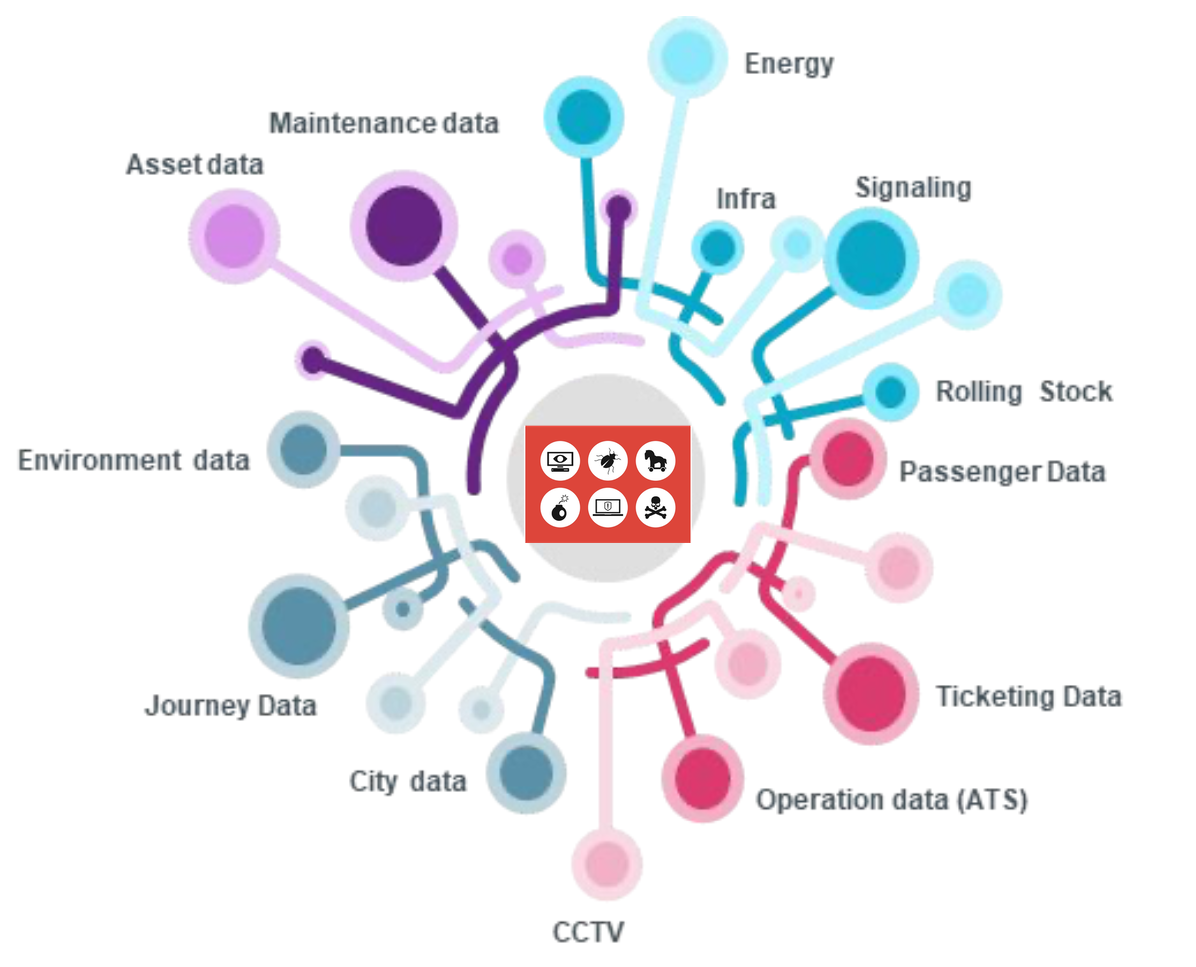
\includegraphics[scale=.17]{gfx/mobilitydata.png}%			\vspace*{-1.2em} 	
		\end{column}
	
		\begin{column}{.45\textwidth}
			\vspace{3em}
			\normalcaption{Adoption of new technologies}
				\begin{itemize}
				\item New connectivity (LTE, Ethernet, \ldots)
				\item Software
				\item New services
				\item IoT
				\item Artificial Intelligence
			\end{itemize}			
		\end{column}	
	\end{columns}
\end{frame}

%%----------------------------------------

\begin{frame}{frame example}
	\framesubtitle{item with subitem}
		\begin{itemize}
			\item Railway-specific challenges need to be addressed
				\begin{itemize}
					\item  Attackers have fairly easy physical access
					\item The train is only one part of an diverse cross-border eco-system
					\item There are safety-critical and non safety-critical systems in the environment
				\end{itemize}
			\item Commercially viable methods for operators, Manufacturers and vendors are needed
			\item Synchronization points between stakeholders as well as safety and security required
		\end{itemize}		
			
\end{frame}
%%----------------------------------------
\begin{frame}{frame example}
	\framesubtitle{item and hightlight}
		\begin{itemize}
			\item Important number of \alert{heterogeneous information systems(s)}
			\item A \alert{wide and distributed} geographical footprint
			\item Limited resources (physical, electrical, connectivity, etc)
			\item Very \alert{long lifecycle} of assets
			\item Importance of legacy
			\item \alert{Reuse of components} not design for railway
			\item \alert{Boundaries} are vanishing
			\item New \alert{passenger-centric} services
		\end{itemize}		
			
\end{frame}
%%----------------------------------------
\begin{frame}{frame example}
	\framesubtitle{full size image}
		\begin{figure}[hbt]
  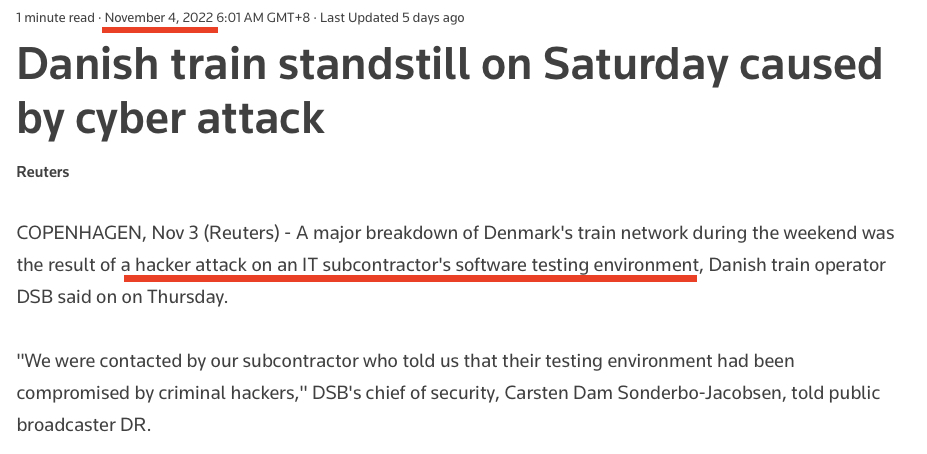
\includegraphics[width=.9\textwidth]{gfx/news.jpeg}
%  \caption{News from REUTERS: Danish train is attacked}
\end{figure}
	
			
\end{frame}
%%----------------------------------------
%%-----------------------------------------

%\begin{frame}[fragile]{Theme Options \& Remarks}
%	\begin{center}
%		\arrayrulecolor{dnvdarkblue}
%		\begin{tabular}[]{lll}
%			\toprule
%			{\bfseries Phase (50126)} 	& {\bfseries Synchronization points and deliverables} & {\bfseries Cybersecurity activities}\\
%			\midrule
%			purple				& switch to {\bfseries\color[RGB]{137,57,94} red purple} colour scheme & \\[0.5em]
%			xcolor={table}		& should be activated to colour tables & \\[0.5em]
%			notheorems			& should be activated to use the dummyblock definition & \\
%			\bottomrule
%		\end{tabular}
%	\end{center}	
%	Note that if you use the
%	\begin{verbatim}  \usepackage{pgfpages}
%  \setbeameroption{show notes on second screen=right}
%  \setbeamertemplate{note page}[compress] \end{verbatim}
%    to enable notes on the second screen there is a bug in beamer that normal text on frames becomes white. So I added a \texttt{dummyblock} wrapper to solve this issue.
%\end{frame}


\section{Section 2}

\begin{frame}{Title\ldots }
\begin{columns}[T]
    \begin{column}{.7\linewidth}
      \begin{itemize}
			\item blabal\ldots blabal\ldots blabal\ldots
				\begin{itemize}
					\item blabal\ldots blabal\ldots
					\item blabal\ldots blabal\ldots blabal\ldots blabal\ldots
					
				\end{itemize}
			\item blabal\ldots blabal\ldots
				\begin{itemize}
					\item blabal\ldots blabal\ldots
					\item blabal\ldots blabal\ldots
					\item blabal\ldots blabal\ldots/ \alert{(OT)} blabal\ldots blabal\ldots 				\end{itemize}
		\end{itemize}
    \end{column}
    \begin{column}{.3\linewidth}
    \begin{figure}[hbt]
  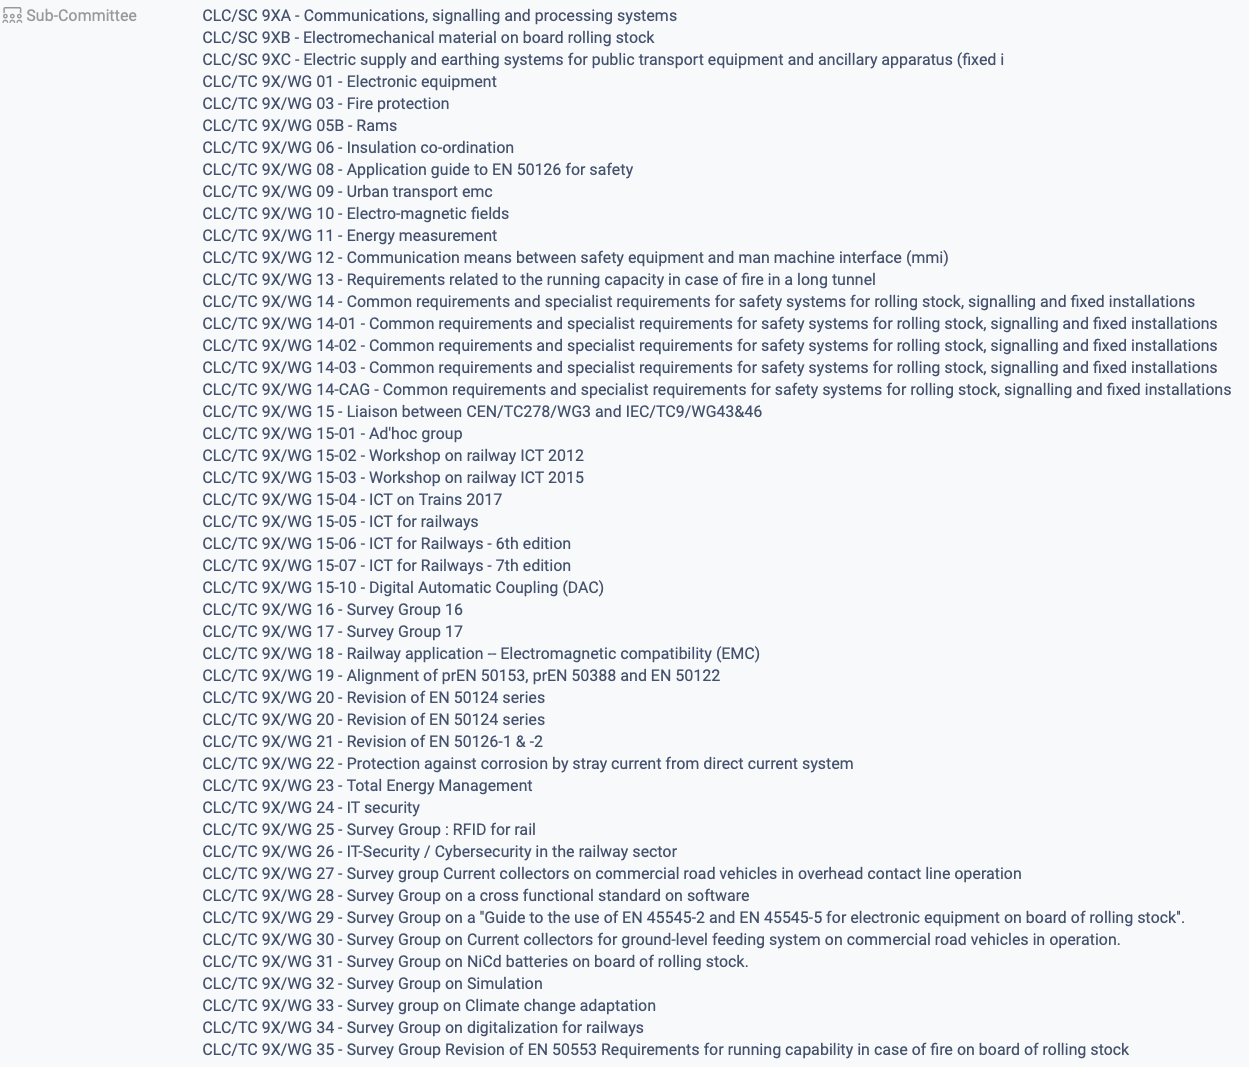
\includegraphics[width=\textwidth]{gfx/standards.jpg}
  \caption{caption}
\end{figure}

    \end{column}  
  \end{columns}
\end{frame}

%%----------------------------------------


%%----------------------------------------
\subsection*{subsection title}
\begin{frame}{Title}
	\framesubtitle{subtitle}
\end{frame}
%%----------------------------------------

\section{section X}
\begin{frame}{Title}
	\framesubtitle{sub title}

	
\end{frame}
%%--------------------------------------------------

%
%%%%%%%%%%%%%%%%%%%%%%%%%%%%%%%%%%%%%%%%%%%%%%%%%%%
%%%%	Blocks, Alerts \& Math Environments
%%%%%%%%%%%%%%%%%%%%%%%%%%%%%%%%%%%%%%%%%%%%%%%%%%%
\section{Blocks}
\begin{frame}{Blocks, Alerts \& Math Environments}
	\begin{block}{Notation}
		This is some notation.
	\end{block}

	\begin{definition}
		This is a definition.
	\end{definition}
	
	\begin{remark}
		And this is a remark.
	\end{remark}
\end{frame}

\begin{frame}
	\begin{theorem}[Existence \& Uniqueness for ...]
		A theorem is important so it should be emphasised!
	\end{theorem}

	\begin{proposition}
		A proposition may be a little less important but it's also worth emphasising!
	\end{proposition}
	
	In the same way we can create lemmata \& corollaries.
\end{frame}

\begin{frame}\label{slide::ex-alert-el}
	\begin{example}
		Examples should be made. Of course normally only the mathematician understands why this text on the blackboard should be an example.
	\end{example}

	Finally
		
	\begin{alertblock}{Alert, alert}
		An alert block has a catchy colour.
	\end{alertblock}
\end{frame}


{
%	\definecolor{dnvdarkblue}{RGB}{137,57,94}
%	\definecolor{dnvgreen}{RGB}{57,137,100}
%	\definecolor{dnvskyblue}{RGB}{255,175,0}
	\begin{frame}{Red purple colour scheme}
		Finally let us have a look at the second colour scheme:
		
		\begin{theorem}[Existence \& Uniqueness for ...]
			A theorem is important so it should be emphasised!
		\end{theorem}
	
		\begin{example}
			Examples should be made. Of course normally only the mathematician understands why this text on the blackboard should be an example.
		\end{example}
	
		\begin{alertblock}{Alert, alert}
			An alert block has a catchy colour.
		\end{alertblock}
	\end{frame}
}


%%%%%%%%%%%%%%%%%%%%%%%%%%%%%%%%%%%%%%%%%%%%%%%%%%%
%%%%	Overlays \& Images
%%%%%%%%%%%%%%%%%%%%%%%%%%%%%%%%%%%%%%%%%%%%%%%%%%%
\section{Overlays \& Images}
\begin{frame}[fragile]
	\frametitle{Overlays \& Images}
	Complying with the old saying: \enquote{A picture speaks a thousand words}, we can create frames which only contain a picture by
	\begin{center}
		\texttt{\textbackslash imageFrame\{imageURL\}.}
	\end{center}
	We can also define an overlay on the left oder right side of the frame. By default the overlay has a width of 150pt. We can adjust as an optional argument.
	\begin{verbatim} \imageFrameOverlayLeft[optional width]{%
    ./gfx/horizontallift.pdf}{%
    Want big impact?}{%
    Use a big picture.} \end{verbatim}
\end{frame}

%%%%	image frame with overlay left
\imageFrameOverlayLeft{%
./gfx/horizontallift.pdf}{%
Want big impact?}{%
Use a big picture.}

%%%%	image frame with overlay right, custom size
\imageFrameOverlayRight[150pt]{%
./gfx/horizontallift.pdf}{%
Need a bigger overlay on the right side?}{%
}


%%%%%%%%%%%%%%%%%%%%%%%%%%%%%%%%%%%%%%%%%%%%%%%%%%%
%%%%	Listings, Tables, Highlighted Text \& Tikz
%%%%%%%%%%%%%%%%%%%%%%%%%%%%%%%%%%%%%%%%%%%%%%%%%%%
\section{Listings, Tables, Highlighted Text \& Tikz}

\begin{frame}{Listings}
	\begin{itemize}
		\item Item $\sharp$1
		\item Item $\sharp$2
			\begin{itemize}
				\item Subitem 2.$\sharp$1
				\item Subitem 2.$\sharp$2
			\end{itemize} 
	\end{itemize}
	and so on. We can also create highlighted lists:
	\begin{itemize}[<+- | alert@+>]
		\item \alert<4>{\only<-3>{Hi!}\only<4>{or here?}}
		\item you
		\item there!
	\end{itemize}
\end{frame}

\begin{frame}{Tables}
	\begin{center}
		\arrayrulecolor{dnvdarkblue}
		\begin{tabular}[]{lrrl}
			\toprule
								& \multicolumn{1}{c}{{\bfseries Dual space}}
			                    & \multicolumn{1}{c}{{\bfseries Reflexive}}
			                    & \multicolumn{1}{l}{{\bfseries Norm}} \\
			\midrule
			$\mathbb K^n$	& $\mathbb K^n$			& Yes			& $\Vert x\Vert_2 =\left(\sum_{i=1}^n |x_i|^2\right)^{\frac 12}$\\[0.5em]
			$\ell_p$			& $\ell_q$				& Yes			& $\Vert x\Vert_p = \left( \sum_{i=1}^\infty |x_i|^p \right)^{\frac 1p}$\\[0.5em]
			$\ell_1$			& $\ell_\infty$			& \alert{No}	& $\Vert x\Vert_1 = \sum_{i=1}^\infty |x_i|$\\[0.5em]
			$\ell_\infty$	& {\small complicated}	& \alert{No}	& $\Vert x\Vert_\infty = \sup_i |x_i|$\\[0.5em]
			$L^p(\mu)$		& $L^q(\mu)$			& Yes			& $\Vert f\Vert_p = \left( \int |f|^p \, \mathrm d\mu \right)^{\frac 1p}$\\[0.5em]
			$L^1(\mu)$		& $L^\infty(\mu)$ 		& \alert{No} 	& $\Vert f\Vert_1 = \int |f| \, \mathrm d\mu$\\
			\bottomrule
		\end{tabular}
	\end{center}
\end{frame}

%%%%%%%%%%%%%%%%%%%%%%%%%%%%%%%%%%%%%%%%%%%%%%%%%%%
%%%%	highlighted frame with number and 
%%%%	optional subtext
%%%%%%%%%%%%%%%%%%%%%%%%%%%%%%%%%%%%%%%%%%%%%%%%%%%
\highlightedFrame[such an impressive number should be big!]{89.432.567}

\begin{frame}{Tikz}
	\begin{center}
	    \begin{tikzpicture}[scale=.8]
	        \pgfmathsetseed{2236}
	
	        \fill (0,0) circle (2pt);
		    \draw (0,0) ellipse (5 and 3);
	    		\node at (5,-2.5) {$D \subsetneq \mathbb R^n$};
	        
	        \draw[decorate, decoration={random steps,segment length=5pt,amplitude=10pt}] [dnvdarkblue] plot [smooth, tension=1] coordinates { (0,0) (2,0) (0,2.5) (-3,0) (0,-1.5) (4,1.8)};
	        \node[dnvdarkblue] at (2.8,-1.5) {BM with $p_t$, $T_t$};
	        
	        \node at (5.2,1.8) {$\partial D \ni x_0$};
	        \fill (4,1.8) circle (1pt);
	        
	        \draw[->,dnvgreen,thick] (4,1.8) -- (3,1);
	        
	        \draw[->,dnvskyblue,thick] (4,1.8) -- (5,2.6);
	        \fill (4,1.8) circle (.5pt);
	    \end{tikzpicture}
	\end{center}
	
	\begin{itemize}
	    \item Trap, $x_0$ absorbing = Killing Brownian motion = Dirichlet problem
	    \item {\color{dnvgreen} Reflected Brownian motion = Neumann problem}
	    \item {\color{dnvskyblue} Wait an go on = Sticky Brownian motion}
	\end{itemize}
\end{frame}





%%%%%%%%%%%%%%%%%%%%%%%%%%%%%%%%%%%%%%%%%%%%%%%%%%%
%%%%	conclusion frame
%%%%%%%%%%%%%%%%%%%%%%%%%%%%%%%%%%%%%%%%%%%%%%%%%%%
\section{Conlusion}
\begin{frame}[fragile]{Conclusion}

%  Let me close addressing some thanks for the inspiration to the \href{https://github.com/matze/mtheme/}{metropolis mtheme}. This theme and its sources \& demo are completely hosted by
%
%  \begin{center}\url{https://github.com/vipowueb/minflat-beamer}\end{center}
%
%  It \emph{itself} is licensed under the
%  \href{http://creativecommons.org/licenses/by-sa/4.0/}{Creative Commons
%  Attribution-ShareAlike 4.0 International License}.

  \begin{center}\ccbysa\end{center}
\end{frame}

%%%%%%%%%%%%%%%%%%%%%%%%%%%%%%%%%%%%%%%%%%%%%%%%%%%
%%%%	thanks slide, not in toc
%%%%%%%%%%%%%%%%%%%%%%%%%%%%%%%%%%%%%%%%%%%%%%%%%%%
\sectionNotInTocAndNavigation{Thanks for your time. Questions?}


\end{document}